% SlideX example deck. Build from this folder:
%   TEXINPUTS=../latex: pdflatex demo.tex   (twice), or open demo.tex in SlideX
%   (File > Open LaTeX Source). Movies need their posters: after a first run,
%   python3 ../latex/slidemovie.py posters demo, then run pdflatex again.
\documentclass[aspectratio=169]{beamer}
\usetheme{default}
\setbeamertemplate{navigation symbols}{}
\setbeamertemplate{footline}[frame number]
\usepackage{slidemovie}   % movies and GIFs that play in SlideX
\usepackage{tcolorbox}
\usepackage{tikz}

\definecolor{ink}{RGB}{28,52,86}
\setbeamercolor{frametitle}{fg=ink}
\setbeamercolor{title}{fg=ink}
\setbeamercolor{structure}{fg=ink}

% A box macro: SlideX can resize each use of it on the preview.
\newcommand{\keybox}[1]{%
	\begin{tcolorbox}[colback=white,colframe=ink,boxsep=1pt,left=6pt,right=6pt,top=4pt,bottom=4pt,width=\linewidth]
		\centering #1
	\end{tcolorbox}}

\title{SlideX example deck}
\subtitle{Movies, overlays, figures, boxes and notes}
\author{SlideX}
\date{}

\begin{document}

\begin{frame}[label=title]
	\titlepage
\end{frame}

\section{Movies}

\begin{frame}[label=movie]{Movies play in place, and keep playing through overlays}
	\begin{columns}[c]
		\column{0.56\linewidth}
		\slidemovie[width=\linewidth]{media/clock.mp4}
		\column{0.4\linewidth}
		\begin{itemize}
			\item<1-> The PDF holds a still image; SlideX plays the movie on top
			\item<2-> This step appears, and the movie does not restart
			\item<3-> Hover the movie for a scrub bar
		\end{itemize}
	\end{columns}
\end{frame}

\begin{frame}[label=options]{Frames, GIFs and playback options}
	\begin{columns}[T]
		\column{0.31\linewidth}\centering
		\slidemovie[width=\linewidth, rate=0.5]{media/sweep.mp4}\\[1mm]
		{\small image frames $\to$ mp4, half speed}
		\column{0.31\linewidth}\centering
		\slidemovie[width=\linewidth]{media/fractal.gif}\\[1mm]
		{\small a GIF, as is}
		\column{0.31\linewidth}\centering
		\slidemovie[width=\linewidth, noautoplay, noloop, start=2, end=4, frame=last]{media/clock.mp4}\\[1mm]
		{\small click to play 2--4 s; the PDF shows 4 s}
	\end{columns}
\end{frame}

\section{Figures}

\begin{frame}[label=figure]{Figures, boxes and captions}
	\begin{columns}[c]
		\column{0.5\linewidth}\centering
		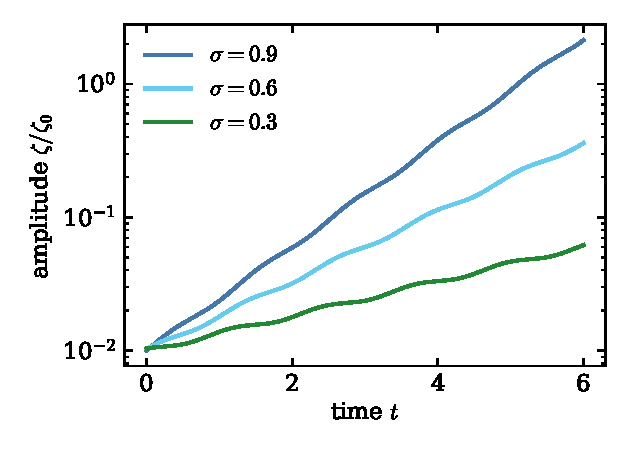
\includegraphics[width=0.95\linewidth]{figures/growth.pdf}\\
		{\small Three modes growing at their own rates}
		\column{0.46\linewidth}
		\begin{tcolorbox}[colback=ink!4,colframe=ink!60,boxrule=0.6pt,arc=1mm,width=\linewidth]
			\begin{itemize}
				\item Exponential growth is a straight line on log axes
				\item The fastest mode overtakes the others early
				\item Rates: $\sigma = 0.9$, $0.6$ and $0.3$
			\end{itemize}
		\end{tcolorbox}
	\end{columns}
\end{frame}

\begin{frame}[label=place]{Placing things}
	\begin{columns}[c]
		\column{0.5\linewidth}\centering
		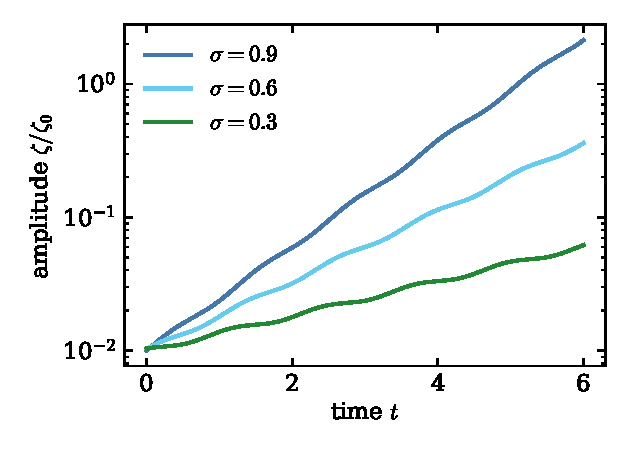
\includegraphics[width=0.9\linewidth]{figures/growth.pdf}
		\column{0.42\linewidth}
		\begin{tcolorbox}[colback=ink!4,colframe=ink!60,boxrule=0.6pt,arc=1mm,width=\linewidth]
			In SlideX, drag the figure or this box up or down, or the gap between the columns
		\end{tcolorbox}
	\end{columns}
	\begin{tikzpicture}[remember picture, overlay]
		\node[fill=ink, text=white, rounded corners=2pt, inner sep=5pt] at ([xshift=-32mm,yshift=-19mm]current page.north east) {A TikZ node: drag it anywhere};
	\end{tikzpicture}
\end{frame}

\begin{frame}[label=keybox]{A box macro, and an equation}
	\keybox{In SlideX, \textbf{double-click any text} on the preview to edit it in place.}
	\vspace{4mm}
	\begin{itemize}
		\item<1-> The amplitude grows as $\zeta(t) = \zeta_0\, e^{\sigma t}$
		\item<2-> so its growth rate is
			\[ \sigma = \frac{1}{\zeta}\,\frac{d\zeta}{dt}. \]
	\end{itemize}
\end{frame}

\appendix
\section*{Backup}

\begin{frame}[label=backup,noframenumbering]{Backup: where the example media came from}
	\begin{itemize}
		\item \texttt{media/clock.mp4}: ffmpeg's \texttt{testsrc2} test pattern
		\item \texttt{media/sweep.mp4}: 24 PNG frames, made with \texttt{slidemovie.py encode}
		\item \texttt{media/fractal.gif}: ffmpeg's \texttt{mandelbrot} source
		\item \texttt{figures/growth.pdf}: \texttt{figures/make\_figures.py}
	\end{itemize}
\end{frame}

\end{document}
